\documentclass[9pt]{beamer}

%!TEX root = ../notas_de_clase.tex

%preamble

 
\usepackage[letterpaper, portrait, margin=0.8in]{geometry}
%language
\usepackage[spanish,es-nodecimaldot]{babel}
\usepackage[utf8]{inputenc}
\usepackage{apacite}



%packages
\usepackage[Algoritmo]{algorithm}
\usepackage{algorithmicx}
\usepackage[noend]{algpseudocode}
\usepackage{mathtools}
\setlength {\marginparwidth }{2cm}
\usepackage{todonotes}
\usepackage{amsbsy}
\usepackage{amssymb}
\usepackage{amsmath,bm}

\usepackage{xcolor}
\providecommand{\red}[1]{\textcolor{red}{\text{#1}}}
\providecommand{\blue}[1]{\textcolor{blue}{\text{#1}}}
\providecommand{\redb}[1]{\textcolor{red}{\textbf{#1}}}
\providecommand{\blueb}[1]{\textcolor{blue}{\textbf{#1}}}
\usepackage{graphicx}
\usepackage{fancybox}
\usepackage{booktabs}
\usepackage{caption}
\usepackage{float}
%\usepackage[longend,ruled,algochapter,linesnumbered,lined,boxed,commentsnumbered,spanish]{algorithm2e}
%\usepackage[algo2e]{algorithm2e}
\usepackage{amssymb}
\usepackage{amstext}
\usepackage{bm}
\usepackage{wrapfig}
\usepackage{subcaption} % para_unsupervised_chapter
% ============= Personal ================
\usepackage{marginnote} 
\renewcommand*{\marginfont}{\color{blue}\sffamily}
% ============= Personal ================

%formatting

\usepackage[export]{adjustbox}

%caption para figuras
\captionsetup[figure]{width=.8\linewidth, font=small,labelfont={bf},name={Fig.},labelsep=period}
\captionsetup[table]{width=.8\linewidth,font=small,labelfont={bf},name={Tabla},labelsep=period}



\ifx\byn\undefined
    \definecolor{my_blue}{HTML}{C2D5FF}
    \definecolor{my_red}{HTML}{FFC2C2}
    \definecolor{my_yellow}{HTML}{FFFFE0}
\else
    \definecolor{my_blue}{HTML}{FFFFFF}
    \definecolor{my_red}{HTML}{FFFFFF}
    \definecolor{my_yellow}{HTML}{FFFFFF}
\fi


\usepackage[framemethod=TikZ]{mdframed}
\mdfdefinestyle{discusion}{%
    %linecolor=black,
    %outerlinewidth=0pt,
    roundcorner=0pt,
    innertopmargin=5pt,
    innerbottommargin=5pt,
    innerrightmargin=20pt,
    innerleftmargin=20pt,
    backgroundcolor=my_blue}

\colorlet{Green}{green!90}


\mdfdefinestyle{ejemplo}{%
    %linecolor=black,
    %outerlinewidth=0pt,
    roundcorner=0pt,
    innertopmargin=5pt,
    innerbottommargin=5pt,
    innerrightmargin=20pt,
    innerleftmargin=20pt,
    backgroundcolor=my_yellow}


\mdfdefinestyle{pendiente}{%
    style = discusion, 
    backgroundcolor=my_red}


\RequirePackage{url}

%definitions
\def\td{{\text d}}
\def\R{{\mathbb R}}
\def\cN{{\mathcal N}}
\def\N{{\mathbb N}}
\def\datos{{\mathcal T}}
\def\eye{{\mathbb I}}
\def\ssum{{\scriptstyle\sum}}
\def\bepsilon{{\bm \epsilon}}
\def\tx{\tilde{x}}
\def\tX{\tilde{X}}
\newcommand{\gp}{\ensuremath{\mathcal{GP}}}
\newcommand{\pr}{\ensuremath{\mathbb{P}}}
\newcommand{\x}{\ensuremath{\mathbf{x}}}
\newcommand{\z}{\ensuremath{\mathbf{z}}}
\newcommand{\cvector}{\ensuremath{\mathbf{c}}}
\newcommand{\e}{\ensuremath{\mathbf{e}}}
\newcommand{\y}{\ensuremath{\mathbf{y}}}
\newcommand{\bx}{\ensuremath{\textcolor{blue}{X}}}
\newcommand{\by}{\ensuremath{\textcolor{blue}{Y}}}
\newcommand{\rx}{\ensuremath{\textcolor{red}{X_*}}}


\DeclareMathOperator*{\argmax}{arg\,max}
\DeclareMathOperator*{\argmin}{arg\,min}
\DeclareMathOperator{\E}{\mathbb{E}}
\DeclareMathOperator{\V}{\mathbb{V}}
\DeclareMathOperator{\KL}{\text{KL}}
\newcommand\deq{\stackrel{\mathclap{\normalfont\mbox{\tiny def}}}{=}}
%\newcommand{\E}[1]{\mathbb E \left[#1\right]}


\usepackage{amsthm}

\newtheorem{theorem}{Theorem}[section]
\newtheorem{corollary}{Corollary}[theorem]
\newtheorem{lemma}[theorem]{Lemma}
\theoremstyle{definition}
\newtheorem{definition}{Definición}[section]



%listing paackage para código
\usepackage{listings}
\usepackage{xcolor}
 
\definecolor{codegreen}{rgb}{0,0.6,0}
\definecolor{codegray}{rgb}{0.5,0.5,0.5}
\definecolor{codepurple}{rgb}{0.58,0,0.82}
\definecolor{backcolour}{rgb}{0.95,0.95,0.92}
 
\lstdefinestyle{mystyle}{
    xleftmargin=0.15\textwidth,
    linewidth=0.8\textwidth,
    backgroundcolor=\color{backcolour},   
    commentstyle=\color{codegreen},
    keywordstyle=\color{magenta},
    numberstyle=\tiny\color{codegray},
    stringstyle=\color{codepurple},
    basicstyle=\ttfamily\footnotesize,
    breakatwhitespace=true,         
    breaklines=true,                 
    captionpos=b,                    
    keepspaces=true,                 
    numbers=left,                    
    numbersep=5pt,                  
    showspaces=false,                
    showstringspaces=false,
    showtabs=false,                  
    tabsize=2
}
 
\lstset{style=mystyle}
\title{\textbf{Aprendizaje de máquinas} \\ Support vector machines (parte 2)}

\begin{document}
\begin{frame}
  \titlepage
\end{frame}

%Método del kernel: motivación.
\begin{frame}{Método del kernel: motivación}

Si bien SVM tiene buenas propiedades de generalización, el método se cae cuando los datos no son linealmente separables. \\~\ \pause

Sin embargo, para la figura de la izquierda, es posible diseñar una característica particular donde los datos sí son linealmente separables. En efecto, consideremos el mapa desde  $\R^2$ a $\R^3$ definido mediante

\begin{equation*}
	\phi: [x_1, x_2]^\top \mapsto [x_1, x_2, x_1 x_2]^\top
\end{equation*}

Esta nueva representación permite separar de forma lineal las clases mediante el plano $z=0$ en $\R^3$ tal como se observa en la figura derecha.

\begin{columns}
\begin{column}{0.5\textwidth}
\begin{figure}[ht]
    \centering
    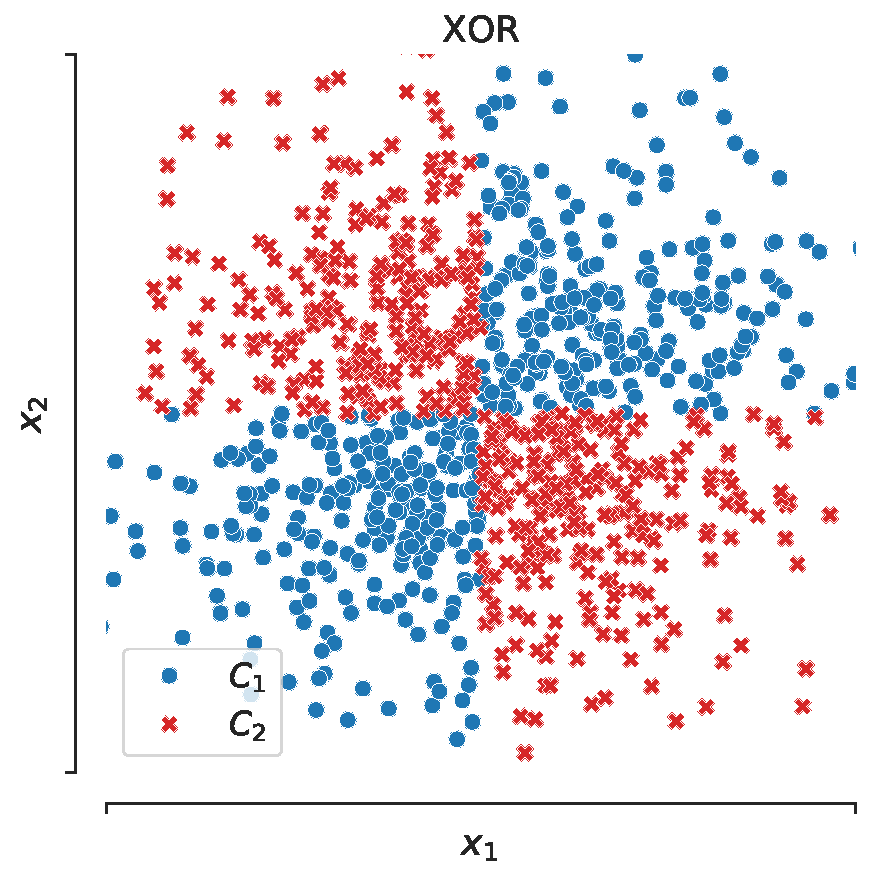
\includegraphics[width=0.6\textwidth]{../img/cap5_xor}
\end{figure}	
\end{column}

\begin{column}{0.5\textwidth}
	
\begin{figure}[ht]
    \centering
    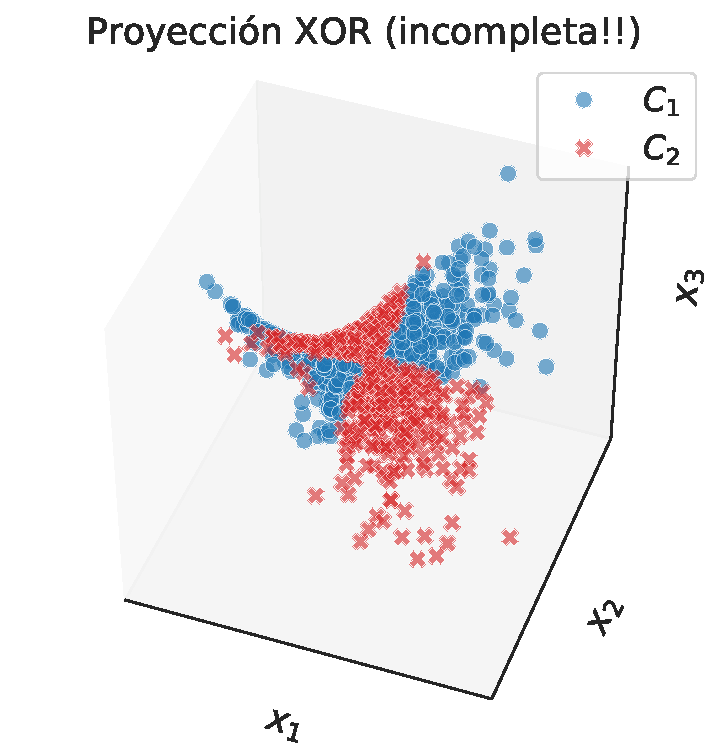
\includegraphics[width=0.6\textwidth]{../img/cap5_xor_3d_proyeccion}
\end{figure}

\end{column}

\end{columns}

\end{frame}

%Método del kernel: idea general.
\begin{frame}{Método del kernel: idea general}

En el caso general no es claro cuál debe ser ``el buen $\phi$''. A pesar de esto, notemos que en la formulación de SVM solo se requiere poder calcular los productos internos entre las características de cada entrada, es decir, si se considera un $\phi$ arbitrario para el problema de clasificación, solo se necesitaría calcular los productos internos de la forma
\begin{equation*}
    \langle \phi(x_i) , \phi(x_j) \rangle
\end{equation*}
 \pause

\begin{columns}


\begin{column}{0.5\textwidth}
	Por lo tanto, si bien no siempre se puede encontrar el $\phi$ exclusivo de cada problema, se puede utilizar uno que sea muy general, esperando que alguno de los términos agregados sea el que efectivamente separa las clases.\\~\ \pause

De esta forma, se puede considerar un mapeo de alta dimensión que incorpore varias combinaciones entre las componentes.

\end{column}
	
\begin{column}{0.5\textwidth}
	\begin{figure}[h]
    \centering
    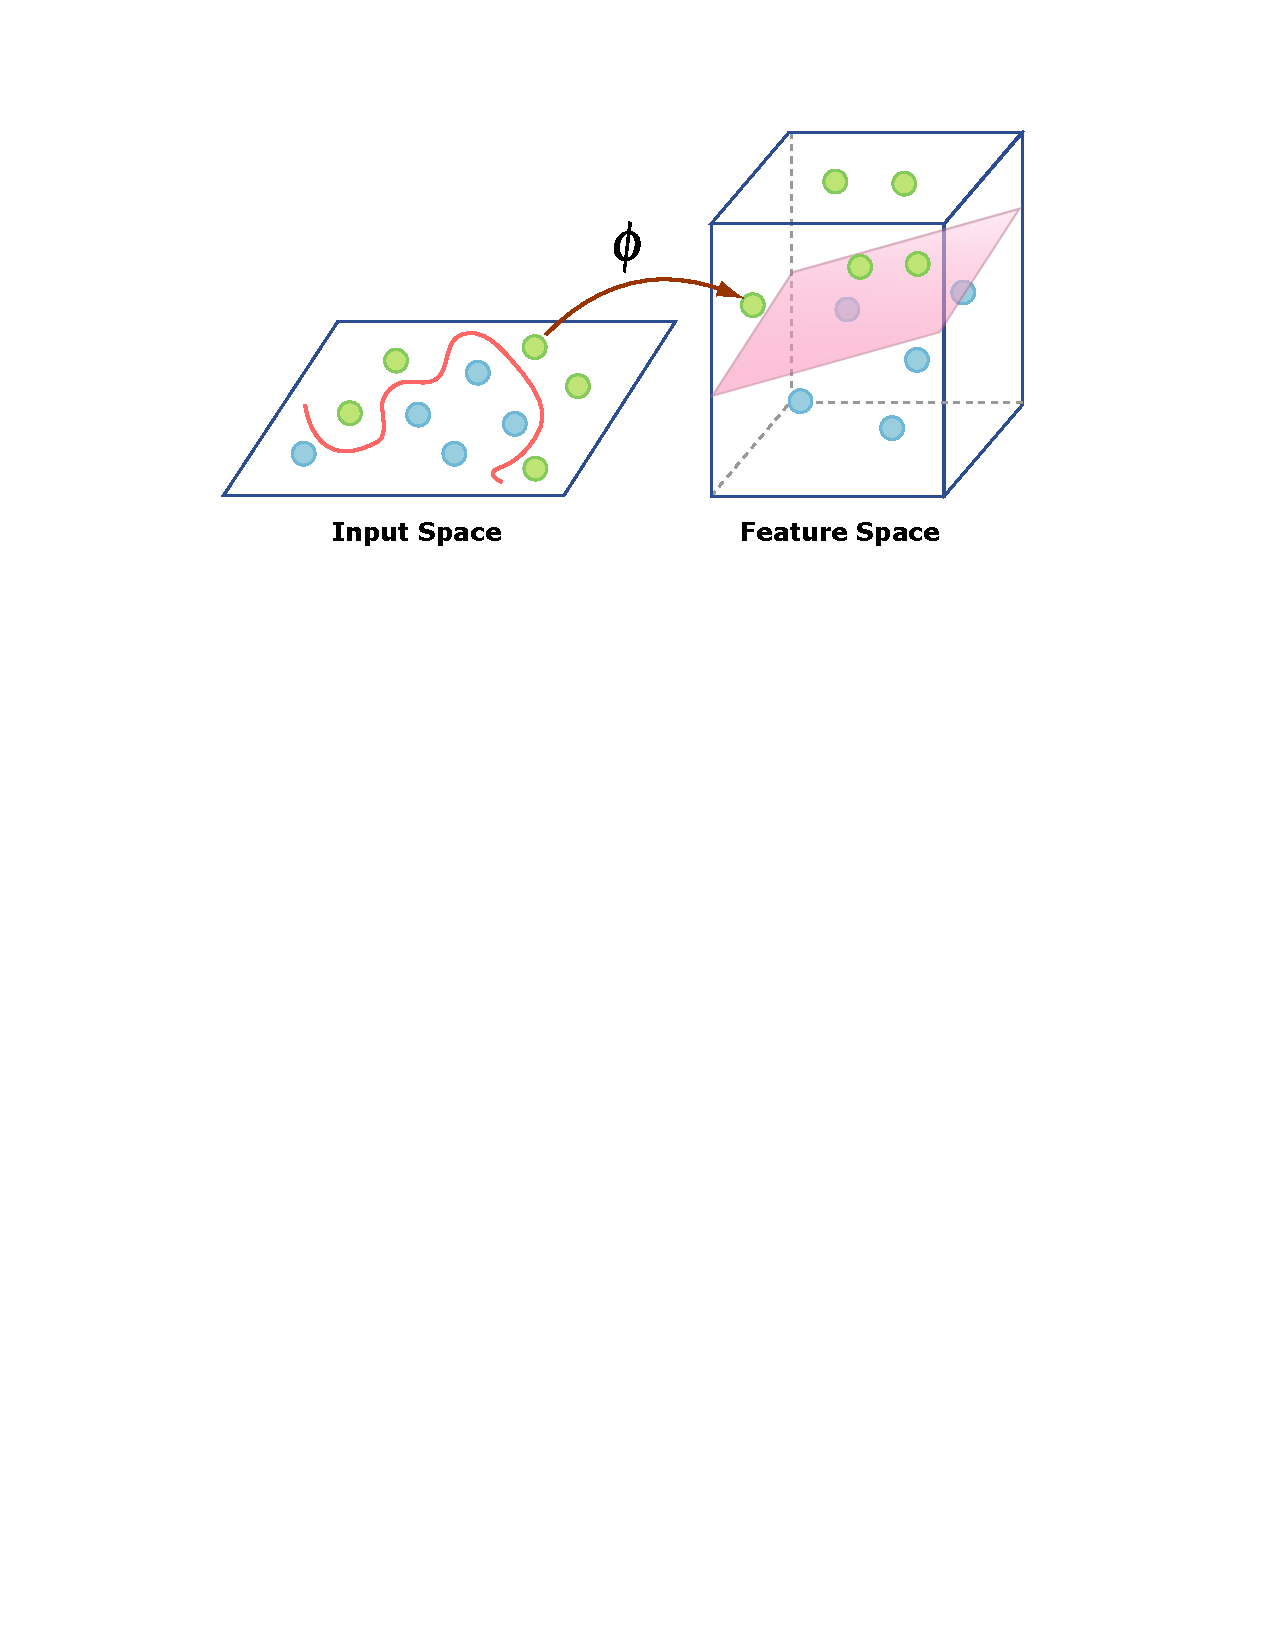
\includegraphics[width=1\textwidth]{../img/cap5_kernelSVM}
\end{figure}
\end{column}	
	
\end{columns}

\end{frame}


%Método del kernel: Mercer kernel.
\begin{frame}{Método del kernel: Mercer kernel}

Para encontrar estos $\phi$ generales, veamos la siguiente definición:

\begin{definition}[Mercer kernel]
    Un Mercer kernel es una función continua $K: X\times X \to \R$ tal que
\begin{itemize}
    \item Es simétrica $K(x_1 , x_2 ) = K (x_2 , x_1)$
    \item Es definida positiva, es decir
    $$\int_{X^2} K(x_1, x_2)g(x_1) g(x_2) dx_1 dx_2\geq 0,$$
    para toda función $g:X\rightarrow\R$ continua. 
\end{itemize}

\end{definition} \pause

El nombre de la segunda propiedad derivada de su similitud con las matrices definidas positivas: si $g$ se mira como vector de $\R^X$, entonces la expresión anterior representa a $g^\top Kg\leq 0$.

\end{frame}

%Método del kernel: teorema de Mercer.
\begin{frame}{Método del kernel: teorema de Mercer}
	De esta forma, se tiene el siguiente teorema de analisis funcional que sustenta la utilización de kernels en los algoritmos de aprendizaje automático:

\begin{theorem}[teorema de Mercer (simplificado)]
	Sea $K: X\times X \to \R$ un Mercer kernel, entonces existe un espacio de Hilbert $\left(\mathcal{H},\langle,\rangle\right)$ y una función $\phi: X \to \mathcal{H}$ tal que:
	\begin{equation*}
    K(x_1, x_2) = \langle \phi(x_1) , \phi(x_2) \rangle
\end{equation*}
\end{theorem} \pause

Es decir, existe un mapa de características $\phi$ tal que $K(x_1, x_2)$ representa el producto interno (en algún espacio) de las características de $x_1$ y $x_2$. Además, dicho espacio no es necesariamente de dimensión finita.
\end{frame}

%Ejemplos de kernels.
\begin{frame}{Ejemplos de kernels}
\textbf{Kernel polinomial:} este kernel está definido por
\begin{equation*}
       K_{pol} (x, y) = (c + x^\top y)^d
\end{equation*}
donde $c\geq 0$ es un parámetro libre y $d\in\N$ es el orden del polinomio. \pause Para el caso $d=2$ se pueden reagrupar los términos para ver que el mapa de características que induce este kernel es
    
\begin{equation*}
        \phi_{pol}(x) = [x_1^2,\ldots,x_m^2,\sqrt{2}x_1x_2,\ldots, \sqrt{2}x_{m}x_{m-1},\sqrt{2c}x_1,\ldots,\sqrt{2c}x_m,c].
\end{equation*}\pause

Es decir, al usar el kernel poliomial se está usando un mapa de características que contiene todos los monomios de grado hasta $d=2$. Esta propiedad se cumple en general para cualquier $d\in\N$.

\end{frame}

%Ejemplos de kernels.
\begin{frame}{Ejemplos de kernels}
\textbf{Función de base radial (RBF kernel):} este kernel también se denomina kernel exponencial cuadrático o gaussiano, y está definido por
    \begin{equation*}
        K_{RBF} (x , y ) = \sigma^2 \exp\left(-\frac{\norm{x -y}^2}{2l^2}\right)
    \end{equation*}
El mapa de características que induce es de dimensión infinita y las fronteras que entrega son suaves (infinitamente diferenciables).\\~\ \pause

\textbf{Kernel periódico:} está definido como
    \begin{equation*}
       K_{per} (x , y) = \sigma^2 \exp\left(- \frac{2\sen^2 \left(\frac{\pi|x -y|}{p}\right)}{l^2}\right).
    \end{equation*}
    
    Este kernel es capaz de rescatar características periódicas en los datos (controlados por el parámetro $p$). 
\end{frame}

%Truco del kernel.
\begin{frame}{Truco del kernel}
	La introducción del concepto de kernel es fundamental en SVM ya que:
	
	\begin{itemize}
		\item El teorema de Mercer afirma que para cualquier función $K$ simétrica y definida positiva, $K(x_1,x_2)$ representa un producto interno en algún espacio de características.\pause
		\item  Dado que SVM solo requiere del cálculo de productos internos, lo anterior permite construir \emph{kernel SVMs}, donde se parametriza directamente el producto interno en el problema de optimización mediante el kernel, pues el teorema de Mercer da la garantía que el mapa de características $\phi$ existe.\pause
		\item Este truco puede aplicarse a cualquier algoritmo en donde las entradas solo aparezcan en la forma de productos punto, proceso que recibe el nombre de \emph{kernelización}. 
	\end{itemize}
	 
\end{frame}

%Kernel SVM.
\begin{frame}{Kernel SVM}

Dado un mapa de características $\phi$, en la formulación de SVM se pueden reemplazar las entadas por las características inducidas por $\phi$. De este modo, el problema primal es:
\begin{equation*}
\begin{aligned}
(P)\quad & \underset{w,b}{\text{min}}
& & \frac{1}{2}||w||^2 + c\sum\limits_{i=1}^{N} \xi_i\\
& \text{s.a}
& & y_i (w^\top \phi(x_i) +b) \geq 1- \xi_i, \; i = 1, \ldots, N.
\end{aligned}
\end{equation*}\pause
Mientras que su formulación dual tiene la forma
\begin{equation*}
\begin{aligned}
(D)\quad & \underset{\alpha}{\text{max}}
& & \sum\limits_{i=1}^{N}\alpha_i - \frac{1}{2} \sum\limits_{i=1}^{N} \alpha_i \alpha_j y_i y_j \langle\phi(x_i), \phi(x_j)\rangle\\
& \text{s.a}
& & \sum\limits_{i=1}^{N} \alpha_i y_i= 0 \\
& &  &0 \leq \alpha_i \leq c
\end{aligned}
\end{equation*}


\end{frame}

%Kernel SVM.
\begin{frame}{Kernel SVM}
	Dado que el problema de optimización solo utiliza los datos mediante productos internos, se puede ocupar el truco del kernel para parametrizar directamente el producto interno $\langle \phi(x_i), \phi(x_j)\rangle$ mediante $K(x_i,x_j)$.\\~\ \pause
	
Con esto, el problema de optimización en el dual se convierte en 
\begin{equation*}
\begin{aligned}
& \underset{\alpha}{\text{max}}
& & \sum\limits_{i=1}^{N}\alpha_i - \frac{1}{2} \sum\limits_{i=1}^{N} \alpha_i \alpha_j y_i y_j K(x_i, x_j)\\
& \text{s.a}
& & \sum\limits_{i=1}^{N} \alpha_i y_i= 0 \\
& &  &0 \leq \alpha_i \leq c
\end{aligned}
\end{equation*}

\end{frame}


%Kernel SVM: ejemplo.
\begin{frame}{Kernel SVM: ejemplo}

La siguiente figura muestra la implementación de kernel SVM para dos kernels:

\begin{itemize}
	\item A la izquierda se utilizó un kernel polinomial de grado $3$
	\item A la derecha se utilizó un kernel un kernel RBF.
\end{itemize}

\begin{figure}[h]
    \centering
    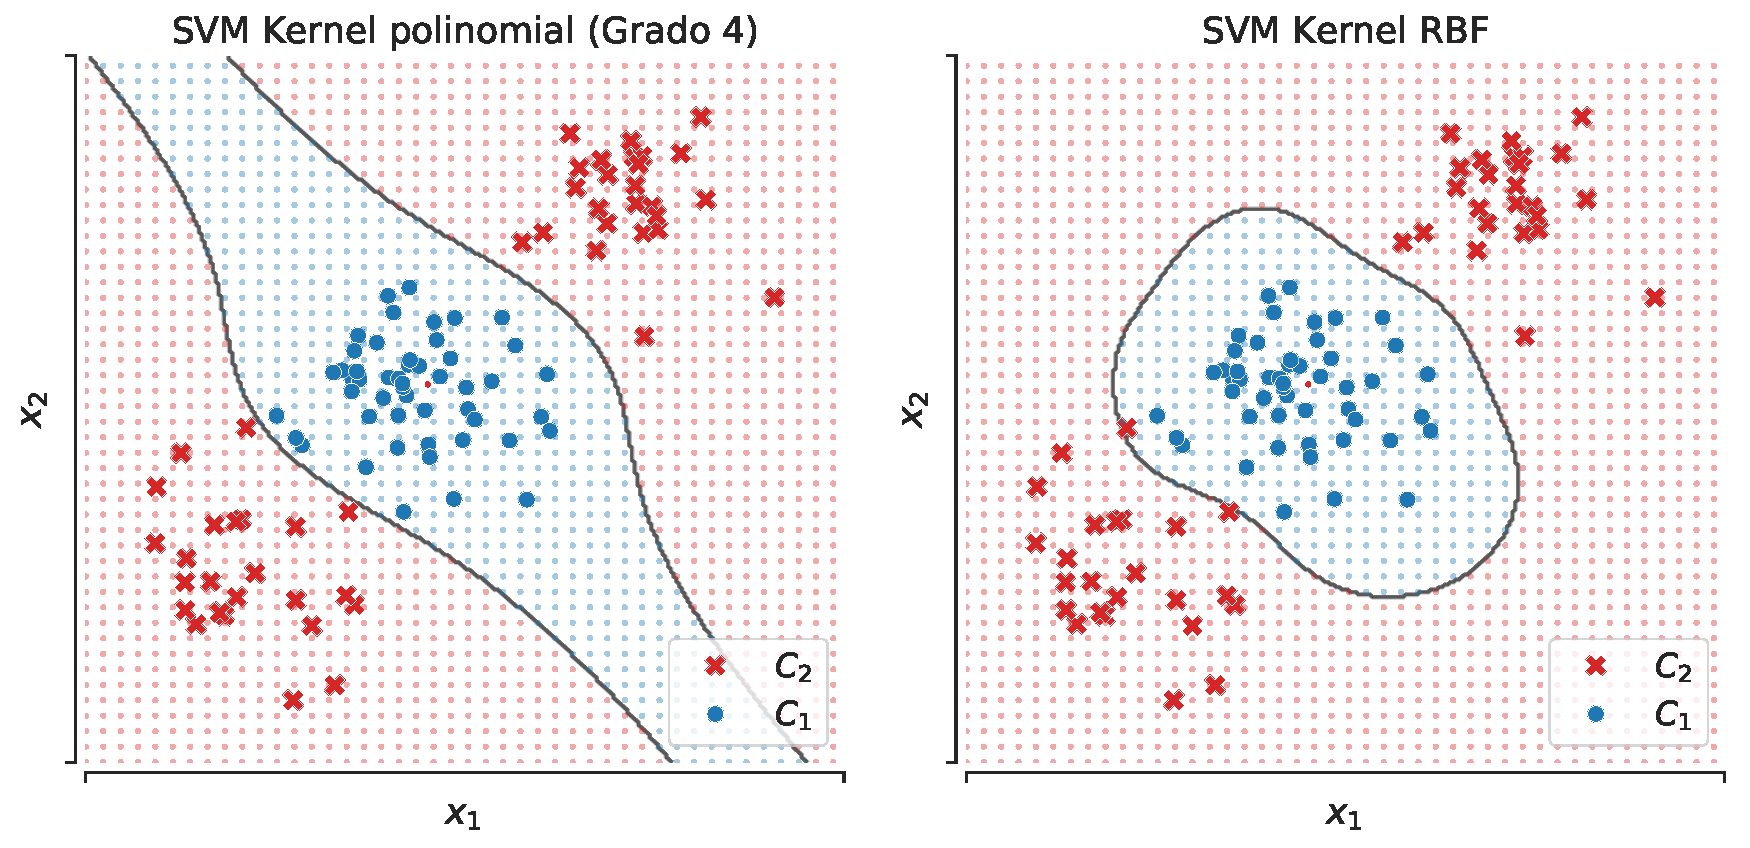
\includegraphics[width=0.8\textwidth]{../img/cap5_svm_2kernels}
\end{figure}

\end{frame}

%Kernel ridge regression.
\begin{frame}{Kernel ridge regression}

Otro método en el que se puede utilizar el truco del kernel es el método de regulación cuadrática usada en regresión lineal, el cual tiene solución
\begin{equation*}
    \theta_{MCR} = \left(\tX^\top\tX +\rho \eye\right)^{-1} \tX^\top Y
\end{equation*}\pause

Si bien las entradas $\tx_i$ no aparecen en forma de producto interno, es posible reescribir la solución de otra forma mediante la fórmula de Woodburry. De este modo se obtiene que

\begin{equation*}
	\theta_{MCR} = \tX^\top\left(\tX\tX^\top + \rho\eye\right)^{-1}Y
\end{equation*}\pause

Ahora $\tX\tX^\top$ sí corresponde a un producto externo de las entradas:

\begin{equation*}
	(\tX\tX^\top)_{ij}=\langle\tX_{i\cdot},\tX^\top_{\cdot j}\rangle=\langle\tX_{i\cdot},\tX_{j\cdot}\rangle = \langle \tx_i,\tx_j\rangle
\end{equation*}\pause

Además, para un nuevo input $x_\star$, su predicción está dada por

\begin{equation*}
	\hat{y}_\star = \theta_{MCR}^\top x_\star = Y^\top \left(\tX\tX^\top + \rho\eye\right)^{-1}\tX \tx_\star
\end{equation*}

donde $(\tX x_\star)_i = \langle \tilde{x}_i,x_\star\rangle$, lo cual muestra que las entradas solo aparecen en la predicción en forma de productos internos.

\end{frame}

%Kernel ridge regression.
\begin{frame}{Kernel ridge regression}

Dado un mapa de características $\phi$, se denotan las características por $\phi_i=\phi(x_i)$ y $\phi_\star = \phi(x_\star)$. De este modo, se puede hacer la regresión sobre las características:

\begin{equation*}
	\Theta=\left(\begin{matrix}
		\phi_1^\top\\
		\vdots\\
		\phi_N^\top
	\end{matrix}\right) \implies \hat{y}_\star = Y^\top \left(\Theta\Theta^\top + \rho\eye\right)^{-1}\Theta \phi_\star
\end{equation*}\pause

Luego, si $K$ es un kernel asociado a $\phi$: $K(x_i,x_j)=\langle\phi(x_i),\phi(x_j)\rangle$, se tiene que


\begin{equation*}
    \hat{y}_\star = Y^\top \left(\Theta\Theta^\top + \rho\eye\right)^{-1}\Theta \phi_\star  = Y^\top \left(K(\tX,\tX) + \rho\eye\right) ^{-1} K(\tX, x_\star),    
\end{equation*}

donde se ha hecho abuso de notación al usar argumentos matriciales en el kernel:
\begin{align*}
	&K(\tX,\tX)_{ij} = (\Theta\Theta^\top)_{ij} = \langle\phi_i,\phi_j\rangle = K(x_i,x_j)\\
	& K(\tX,x_\star)_i = (\Theta\phi_\star)_i = \langle\phi_i,\phi_\star\rangle = K(x_i,x_\star)
\end{align*}
	
\end{frame}


\end{document}
